\documentclass[a4paper,11pt]{article}

% ── Packages ──────────────────────────────────────────────────────────────
\usepackage[utf8]{inputenc}
\usepackage[T1]{fontenc}
\usepackage[margin=2.5cm]{geometry}
\usepackage{amsmath, amssymb}
\usepackage{siunitx}
\usepackage{booktabs}
\usepackage{graphicx}
\usepackage{hyperref}
\usepackage{enumitem}
\usepackage{float}
\usepackage{caption}
\usepackage{xcolor}
\usepackage{fancyhdr}
\usepackage{tikz}

\usetikzlibrary{arrows.meta, positioning, calc}

% ── Header / Footer ──────────────────────────────────────────────────────
\pagestyle{fancy}
\fancyhf{}
\lhead{F1/10th Vehicle Parameter Measurement}
\rhead{Bachelor Project}
\cfoot{\thepage}

% ── Convenience commands ─────────────────────────────────────────────────
\newcommand{\param}[1]{\texttt{#1}}
\newcommand{\note}[1]{\textbf{Note:} #1}
\newcommand{\result}[1]{\begin{center}\fbox{\parbox{0.85\linewidth}{#1}}\end{center}}
\sisetup{per-mode=symbol}

% ── Title ─────────────────────────────────────────────────────────────────
\title{%
  Vehicle Parameter Measurement Test Procedure\\[4pt]
  \large F1/10th — Traxxas Slash 4$\times$4 Chassis%
}
\author{Bachelor Project}
\date{\today}

\begin{document}
\maketitle
\tableofcontents
\newpage

%==========================================================================
\section{Introduction}
%==========================================================================

This document defines the full test procedure for physically measuring every
relevant parameter of the F1/10th platform.  All measurements are performed
on the bare \textbf{Traxxas Slash 4$\times$4} chassis equipped with
\emph{only} the battery and motor (Traxxas 3351R).  The ESC and RC receiver
have been removed and are \emph{not} present during these measurements.

The measured values feed directly into:
\begin{itemize}
  \item The MPC vehicle model (\texttt{mpc\_types.h}, \texttt{vehicle\_model.h})
  \item The planning pipeline (\texttt{vehicle\_params.yaml})
  \item The ROS\,2 control stack (\texttt{vesc.yaml}, EKF parameters)
\end{itemize}

%==========================================================================
\section{Required Equipment}
%==========================================================================

\begin{itemize}
  \item Digital kitchen/postal scale — resolution $\leq\SI{1}{\gram}$
        (range $\geq\SI{5}{\kilo\gram}$)
  \item Vernier caliper or digital caliper — resolution \SI{0.01}{\milli\metre}
  \item Steel ruler or measuring tape — \SI{1}{\metre}, \SI{1}{\milli\metre} graduation
  \item Set square / right-angle tool
  \item Flat, level surface (table)
  \item Pencil / marker
  \item Masking tape
  \item Spirit level (optional, for verifying surface is flat)
  \item 4 small identical blocks or coins (for lifting individual wheels)
\end{itemize}

\note{The vehicle is weighed with the Traxxas 4$\times$4 Slash chassis
containing \textbf{only} the battery and motor.  No ESC, no receiver, no
LiDAR, no compute stack.  Once these components are added later, the
measurements in Section~\ref{sec:mass} should be repeated.}

%==========================================================================
\section{Vehicle Diagram and Nomenclature}
%==========================================================================

The following conventions are used throughout.

\begin{figure}[H]
\centering
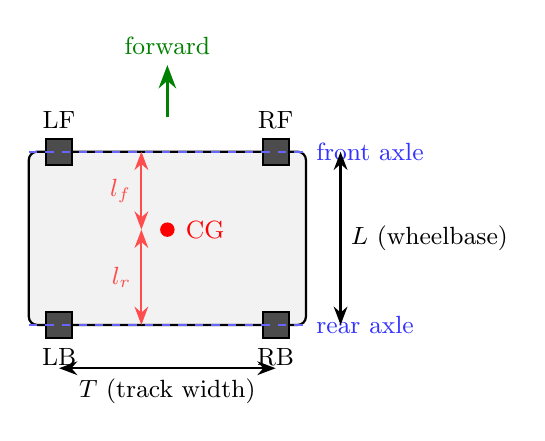
\begin{tikzpicture}[>=Stealth, thick, scale=1.1]
  % Chassis rectangle
  \draw[rounded corners=3pt, fill=gray!10]
    (-1.6, -1.0) rectangle (1.6, 1.0);

  % Wheels
  \filldraw[fill=black!70] (-1.4,  0.85) rectangle (-1.1,  1.15); % LF
  \filldraw[fill=black!70] ( 1.1,  0.85) rectangle ( 1.4,  1.15); % RF
  \filldraw[fill=black!70] (-1.4, -1.15) rectangle (-1.1, -0.85); % LB
  \filldraw[fill=black!70] ( 1.1, -1.15) rectangle ( 1.4, -0.85); % RB

  % Labels on wheels
  \node[above] at (-1.25, 1.15) {\small LF};
  \node[above] at ( 1.25, 1.15) {\small RF};
  \node[below] at (-1.25,-1.15) {\small LB};
  \node[below] at ( 1.25,-1.15) {\small RB};

  % Axle lines
  \draw[dashed, blue!60] (-1.6, 1.0) -- (1.6, 1.0)
    node[right, text=blue!80]{\small front axle};
  \draw[dashed, blue!60] (-1.6,-1.0) -- (1.6,-1.0)
    node[right, text=blue!80]{\small rear axle};

  % Wheelbase
  \draw[<->] (2.0, 1.0) -- (2.0, -1.0)
    node[midway, right]{\small $L$ (wheelbase)};

  % Track width
  \draw[<->] (-1.25, -1.5) -- (1.25, -1.5)
    node[midway, below]{\small $T$ (track width)};

  % CG
  \filldraw[red] (0, 0.1) circle (2pt) node[right=3pt]{\small CG};

  % Lf, Lr
  \draw[<->, red!70] (-0.3, 1.0) -- (-0.3, 0.1)
    node[midway, left]{\small $l_f$};
  \draw[<->, red!70] (-0.3,-1.0) -- (-0.3, 0.1)
    node[midway, left]{\small $l_r$};

  % Direction arrow
  \draw[->, very thick, green!50!black] (0, 1.4) -- (0, 2.0)
    node[above]{\small forward};
\end{tikzpicture}
\caption{Top-down schematic with parameter naming conventions.}
\label{fig:vehicle_layout}
\end{figure}

\begin{table}[H]
\centering
\caption{Parameter symbols and descriptions.}
\label{tab:symbols}
\begin{tabular}{@{}lll@{}}
\toprule
\textbf{Symbol}    & \textbf{Parameter}                         & \textbf{Unit}\\
\midrule
$m$                & Total vehicle mass                         & \si{\kilo\gram}\\
$m_\text{LF}$      & Mass on left-front wheel                  & \si{\kilo\gram}\\
$m_\text{RF}$      & Mass on right-front wheel                 & \si{\kilo\gram}\\
$m_\text{LB}$      & Mass on left-rear wheel                   & \si{\kilo\gram}\\
$m_\text{RB}$      & Mass on right-rear wheel                  & \si{\kilo\gram}\\
$L$                & Wheelbase (front-to-rear axle)            & \si{\metre}\\
$l_f$              & Distance from CG to front axle            & \si{\metre}\\
$l_r$              & Distance from CG to rear axle             & \si{\metre}\\
$T_f$              & Front track width (centre-to-centre)      & \si{\metre}\\
$T_r$              & Rear track width (centre-to-centre)       & \si{\metre}\\
$d_w$              & Wheel (tire) outer diameter               & \si{\metre}\\
$r_w$              & Wheel (tire) rolling radius               & \si{\metre}\\
$w_t$              & Tire width                                & \si{\metre}\\
$h_\text{cg}$      & Centre-of-gravity height                  & \si{\metre}\\
$L_\text{total}$   & Overall vehicle length                    & \si{\metre}\\
$W_\text{total}$   & Overall vehicle width                     & \si{\metre}\\
$I_z$              & Yaw moment of inertia                     & \si{\kilo\gram\metre\squared}\\
\bottomrule
\end{tabular}
\end{table}

%==========================================================================
\section{Test~1: Mass and Weight Distribution}
\label{sec:mass}
%==========================================================================

\subsection{Purpose}
Determine the total mass $m$ and the individual corner weights
$m_\text{LF}$, $m_\text{RF}$, $m_\text{LB}$, $m_\text{RB}$.  From
these, the longitudinal CG position ($l_f$, $l_r$) and the lateral
CG offset are computed.

\subsection{Setup}
\begin{enumerate}
  \item Place the scale on a flat, level surface.
  \item Set wheels straight ahead (zero steering angle).
  \item The vehicle contains \textbf{only} the battery and motor —
        verify that no ESC or receiver is installed.
\end{enumerate}

\subsection{Procedure}

\subsubsection{Individual corner weights}
The total mass is derived from the sum of all four corner weights,
so no separate whole-vehicle weighing step is needed.  (An independent
total-mass measurement can be added later as a verification.)

\noindent For each corner (LF, RF, LB, RB):
\begin{enumerate}
  \item Place \emph{one} wheel on the scale.
  \item Support the other three wheels at the \emph{same} height as the
        scale surface (use spacer blocks of identical thickness so the
        chassis is level).
  \item Record the reading as $m_\text{XX}$.
  \item Repeat for all four corners.
\end{enumerate}

\note{When an independent total-mass measurement becomes available,
verify that $m_\text{LF}+m_\text{RF}+m_\text{LB}+m_\text{RB}
\approx m$.  Any deviation $>\SI{2}{\percent}$ indicates the chassis
was not level during corner weighing.}

\subsection{Data Recording}

\result{%
\begin{tabular}{@{}ll@{}}
\toprule
\textbf{Quantity} & \textbf{Measured value}\\
\midrule
$m_\text{LF}$ & \SI{0.572}{\kilo\gram}\\
$m_\text{RF}$ & \SI{0.501}{\kilo\gram}\\
$m_\text{LB}$ & \SI{0.604}{\kilo\gram}\\
$m_\text{RB}$ & \SI{0.616}{\kilo\gram}\\
\midrule
$m = \sum m_i$ & \SI{2.293}{\kilo\gram} \quad(computed)\\
\bottomrule
\end{tabular}%
}

\subsection{Derived quantities}

Front axle mass and rear axle mass:
\begin{align}
  m_f &= m_\text{LF} + m_\text{RF}, &
  m_r &= m_\text{LB} + m_\text{RB}
\end{align}

Longitudinal CG position (requires wheelbase $L$ from Test~2):
\begin{align}
  l_r &= \frac{m_f}{m}\,L, &
  l_f &= L - l_r
  \label{eq:cg_long}
\end{align}

Lateral CG offset from centreline:
\begin{equation}
  \Delta y_\text{cg} =
  \frac{(m_\text{RF}+m_\text{RB}) - (m_\text{LF}+m_\text{LB})}{m}
  \;\cdot\;\frac{T}{2}
  \label{eq:cg_lat}
\end{equation}
where $T$ is the average track width.  A positive value means the CG
is offset to the right.

%==========================================================================
\section{Test~2: Wheelbase}
\label{sec:wheelbase}
%==========================================================================

\subsection{Purpose}
Measure the wheelbase $L$, the distance between the front and rear axle
centres.

\subsection{Procedure}
\begin{enumerate}
  \item Place the vehicle on a flat surface with wheels straight ahead.
  \item Mark the \textbf{centre of the front axle} on the ground
        (midpoint between the two front wheel hubs, projected vertically
        downward; a plumb line or set square helps).
  \item Mark the \textbf{centre of the rear axle} in the same manner.
  \item Measure the distance between the two marks with a caliper or
        ruler.
  \item Repeat 3 times and take the average.
\end{enumerate}

\noindent\textbf{Alternative (direct hub-to-hub):}
Measure from the centre of a front wheel hub to the centre of the
corresponding rear wheel hub on the same side.  Repeat on both sides;
they should agree within \SI{1}{\milli\metre}.

\subsection{Data Recording}

\result{%
\begin{tabular}{@{}ll@{}}
\toprule
\textbf{Measurement} & \textbf{Value}\\
\midrule
$L$  & \SI{0.326}{\metre}\\
\bottomrule
\end{tabular}%
}

Now compute $l_f$ and $l_r$ using Eq.~\eqref{eq:cg_long} and the masses
from Test~1.

\result{%
\begin{tabular}{@{}ll@{}}
\toprule
$l_f$ & \SI{0.1734}{\metre}\\
$l_r$ & \SI{0.1526}{\metre}\\
\bottomrule
\end{tabular}%
}

%==========================================================================
\section{Test~3: Track Width (Front and Rear)}
\label{sec:track}
%==========================================================================

\subsection{Purpose}
Measure the distance between the left and right wheel contact-patch
centres on each axle.

\subsection{Procedure}
\begin{enumerate}
  \item Set wheels straight ahead.
  \item \textbf{Front track $T_f$:} Measure the distance between the
        centres of the two front tyres at ground level (contact-patch
        centre to contact-patch centre).  Alternatively, measure
        hub-to-hub if the wheels are symmetric.
  \item \textbf{Rear track $T_r$:} Same for the rear axle.
  \item Repeat 3 times each.
\end{enumerate}

\subsection{Data Recording}

\result{%
\begin{tabular}{@{}ll@{}}
\toprule
\textbf{Measurement} & \textbf{Value}\\
\midrule
$T_f$  & \SI{0.231}{\metre}\\
$T_r$  & \SI{0.231}{\metre}\\
\bottomrule
\end{tabular}%
}

%==========================================================================
\section{Test~4: Wheel and Tyre Dimensions}
\label{sec:wheel}
%==========================================================================

\subsection{Purpose}
Measure wheel diameter $d_w$, rolling radius $r_w$, and tyre width $w_t$.

\subsection{Procedure}

\subsubsection{Wheel diameter}
\begin{enumerate}
  \item Remove one wheel from the vehicle.
  \item Using a caliper, measure the outer tyre diameter at three
        orientations (rotate \SI{60}{\degree} between measurements)
        to account for out-of-round.
  \item Record the average as $d_w$.
\end{enumerate}

\subsubsection{Rolling radius (loaded)}
\begin{enumerate}
  \item Place the vehicle on a flat surface (all four wheels on the ground,
        full weight applied).
  \item Measure the height from the ground to the centre of a wheel hub
        (use a caliper or ruler against the axle).
  \item This is the \textbf{loaded rolling radius} $r_w$.
  \item Repeat for all four wheels and average.
\end{enumerate}

\note{The loaded rolling radius is generally slightly smaller than
$d_w/2$ due to tyre deformation under load.  The rolling radius is the
value needed for ERPM-to-speed conversion.}

\subsubsection{Tyre width}
\begin{enumerate}
  \item With the wheel removed, measure the tread width (ground contact
        width) with a caliper.
  \item Record as $w_t$.
\end{enumerate}

\subsection{Data Recording}

\result{%
\begin{tabular}{@{}ll@{}}
\toprule
\textbf{Measurement} & \textbf{Value}\\
\midrule
$d_w$                  & \SI{0.100}{\metre}\\
\midrule
$r_w$ (loaded, LF)     & \SI{0.0500}{\metre}\\
$r_w$ (loaded, RF)     & \SI{0.0505}{\metre}\\
$r_w$ (loaded, LB)     & \SI{0.0505}{\metre}\\
$r_w$ (loaded, RB)     & \SI{0.0505}{\metre}\\
$r_w$ (average)         & \SI{0.05038}{\metre}\\
\midrule
$w_t$                   & \SI{0.043}{\metre}\\
\bottomrule
\end{tabular}%
}

%==========================================================================
\section{Test~5: Overall Dimensions}
\label{sec:overall}
%==========================================================================

\subsection{Purpose}
Measure the overall vehicle length and width for collision avoidance
margins.

\subsection{Procedure}
\begin{enumerate}
  \item \textbf{Overall length $L_\text{total}$:} Measure from the
        furthest-forward point (front bumper) to the furthest-rearward
        point (rear bumper), parallel to the longitudinal axis.
  \item \textbf{Overall width $W_\text{total}$:} Measure the widest
        point of the vehicle (typically the outer edges of the tyres).
\end{enumerate}

\subsection{Data Recording}

\result{%
\begin{tabular}{@{}ll@{}}
\toprule
\textbf{Measurement} & \textbf{Value}\\
\midrule
$L_\text{total}$  & \SI{0.510}{\metre}\\
$W_\text{total}$  & \SI{0.271}{\metre}\\
\bottomrule
\end{tabular}%
}

%==========================================================================
\section{Test~6: Centre-of-Gravity Height}
\label{sec:cg_height}
%==========================================================================

\subsection{Purpose}
Estimate the CG height $h_\text{cg}$ above the ground.  This is needed
for load-transfer calculations and rollover analysis.

\subsection{Method — Tilt Test}

\begin{enumerate}
  \item Place the vehicle on a flat, level surface.
  \item Measure and record the rear-axle weight $m_r^\text{level} =
        m_\text{LB}+m_\text{RB}$ (from Test~1).
  \item Raise the \textbf{front axle} by a known height $\Delta h$ using
        a block or stack of known thickness.  Keep the rear wheels on
        the scale.
  \item Record the new rear-axle scale reading $m_r^\text{tilted}$.
  \item Compute the tilt angle:
        \begin{equation}
          \theta = \arcsin\!\left(\frac{\Delta h}{L}\right)
        \end{equation}
  \item Compute CG height:
        \begin{equation}
          h_\text{cg} = \frac{(m_r^\text{tilted}-m_r^\text{level})\,L}
                             {m\,\tan\theta}
                        \;+\; r_w
          \label{eq:cg_height}
        \end{equation}
        (The $+\,r_w$ accounts for the fact that the axle is one wheel
        radius above the ground.)
\end{enumerate}

\note{Use a tilt of roughly \SIrange{5}{15}{\degree} for best accuracy.
Too small and the weight shift is in the noise; too large and the
battery may shift.}

\subsection{Data Recording}

\result{%
\begin{tabular}{@{}ll@{}}
\toprule
\textbf{Quantity} & \textbf{Value}\\
\midrule
$\Delta h$ (front raised)      & \rule{3cm}{0.4pt}~\si{\metre}\\
$\theta$                       & \rule{3cm}{0.4pt}~\si{\degree}\\
$m_r^\text{level}$             & \rule{3cm}{0.4pt}~\si{\kilo\gram}\\
$m_r^\text{tilted}$            & \rule{3cm}{0.4pt}~\si{\kilo\gram}\\
\midrule
$h_\text{cg}$ (computed)       & \rule{3cm}{0.4pt}~\si{\metre}\\
\bottomrule
\end{tabular}%
}

%==========================================================================
\section{Test~7: Yaw Moment of Inertia (Estimation)}
\label{sec:inertia}
%==========================================================================

\subsection{Purpose}
Estimate the yaw moment of inertia $I_z$ about the vertical axis through
the CG.

\subsection{Method~A — Bifilar (Two-String) Pendulum}

This is the most practical method for a small vehicle.

\begin{enumerate}
  \item Suspend the vehicle from two parallel strings of equal length
        $l_s$, attached at two points on the chassis separated by a
        horizontal distance $2d$ (symmetric about the CG).
  \item Allow the vehicle to oscillate in yaw (twist about the vertical
        axis) with a small amplitude ($<\SI{10}{\degree}$).
  \item Time $N\geq10$ oscillation periods and compute the average period
        $T_\text{osc}$.
  \item Calculate:
        \begin{equation}
          I_z = \frac{m\,g\,d^2\,T_\text{osc}^2}{4\,\pi^2\,l_s}
          \label{eq:Iz_bifilar}
        \end{equation}
\end{enumerate}

\subsection{Method~B — Compound Pendulum (simpler)}

\begin{enumerate}
  \item Suspend the vehicle from a single pivot point (e.g.\ a bolt
        through a convenient hole) at a known distance $R$ from the CG.
  \item Let it swing as a compound pendulum in the yaw plane and
        measure the period $T_\text{osc}$.
  \item Calculate:
        \begin{equation}
          I_z = \frac{m\,g\,R\,T_\text{osc}^2}{4\,\pi^2} - m\,R^2
          \label{eq:Iz_compound}
        \end{equation}
\end{enumerate}

\subsection{Data Recording}

\result{%
\begin{tabular}{@{}ll@{}}
\toprule
\textbf{Quantity} & \textbf{Value}\\
\midrule
Method used        & \rule{3cm}{0.4pt}\\
$l_s$ or $R$       & \rule{3cm}{0.4pt}~\si{\metre}\\
$d$ (bifilar)      & \rule{3cm}{0.4pt}~\si{\metre}\\
Oscillations $N$   & \rule{3cm}{0.4pt}\\
Total time         & \rule{3cm}{0.4pt}~\si{\second}\\
$T_\text{osc}$     & \rule{3cm}{0.4pt}~\si{\second}\\
\midrule
$I_z$ (computed)   & \rule{3cm}{0.4pt}~\si{\kilo\gram\metre\squared}\\
\bottomrule
\end{tabular}%
}

%==========================================================================
\section{Test~8: Steering Geometry}
\label{sec:steering}
%==========================================================================

\subsection{Purpose}
Measure the maximum mechanical steering angle and characterise the
Ackermann steering geometry.

\subsection{Procedure}

\subsubsection{Maximum steering angle}
\begin{enumerate}
  \item With the servo/steering linkage connected (but no ESC powered),
        manually turn the front wheels to full lock in each direction.
  \item Using a protractor or by measuring geometry (see below),
        determine the maximum steering angle $\delta_\text{max}$ for
        both left and right.
\end{enumerate}

\noindent\textbf{Geometric method for steering angle:}
\begin{enumerate}
  \item Set wheels to full lock.
  \item Mark a straight reference line along the chassis centreline on
        the ground.
  \item Mark the line along the wheel's longitudinal axis (use a ruler
        against the tyre sidewall).
  \item The angle between these two lines is $\delta$.
\end{enumerate}

\subsubsection{Ackermann check}
\begin{enumerate}
  \item At full lock, measure the inner wheel angle $\delta_\text{in}$
        and the outer wheel angle $\delta_\text{out}$.
  \item For perfect Ackermann geometry:
        \begin{equation}
          \cot\delta_\text{out} - \cot\delta_\text{in}
          = \frac{T_f}{L}
        \end{equation}
  \item Record both angles to characterise the actual Ackermann
        percentage.
\end{enumerate}

\subsection{Data Recording}

\result{%
\begin{tabular}{@{}ll@{}}
\toprule
\textbf{Measurement} & \textbf{Value}\\
\midrule
$\delta_\text{max,left}$   & \rule{3cm}{0.4pt}~\si{\degree} (\rule{2cm}{0.4pt}~\si{\radian})\\
$\delta_\text{max,right}$  & \rule{3cm}{0.4pt}~\si{\degree} (\rule{2cm}{0.4pt}~\si{\radian})\\
$\delta_\text{in}$ (full lock)  & \rule{3cm}{0.4pt}~\si{\degree}\\
$\delta_\text{out}$ (full lock) & \rule{3cm}{0.4pt}~\si{\degree}\\
\bottomrule
\end{tabular}%
}

%==========================================================================
\section{Summary of Results}
\label{sec:summary}
%==========================================================================

Transfer all final measured and computed values here.

\begin{table}[H]
\centering
\caption{Complete vehicle parameter summary (Traxxas Slash 4$\times$4,
battery + motor only, no ESC/receiver).}
\label{tab:summary}
\begin{tabular}{@{}llll@{}}
\toprule
\textbf{Parameter} & \textbf{Symbol} & \textbf{Value}
  & \textbf{Config field}\\
\midrule
Total mass                & $m$            & \SI{2.293}{\kilo\gram}
  & \param{mass}\\
Front-left corner mass    & $m_\text{LF}$  & \SI{0.572}{\kilo\gram}
  & —\\
Front-right corner mass   & $m_\text{RF}$  & \SI{0.501}{\kilo\gram}
  & —\\
Rear-left corner mass     & $m_\text{LB}$  & \SI{0.604}{\kilo\gram}
  & —\\
Rear-right corner mass    & $m_\text{RB}$  & \SI{0.616}{\kilo\gram}
  & —\\
\midrule
Wheelbase                 & $L$            & \SI{0.326}{\metre}
  & \param{wheelbase}\\
CG to front axle          & $l_f$          & \SI{0.1734}{\metre}
  & \param{lf}\\
CG to rear axle           & $l_r$          & \SI{0.1526}{\metre}
  & \param{lr}\\
Front track width         & $T_f$          & \SI{0.231}{\metre}
  & —\\
Rear track width          & $T_r$          & \SI{0.231}{\metre}
  & —\\
\midrule
Wheel diameter            & $d_w$          & \SI{0.100}{\metre}
  & —\\
Rolling radius            & $r_w$          & \SI{0.05038}{\metre}
  & —\\
Tyre width                & $w_t$          & \SI{0.043}{\metre}
  & —\\
\midrule
Overall length            & $L_\text{total}$  & \SI{0.510}{\metre}
  & \param{length}\\
Overall width             & $W_\text{total}$  & \SI{0.271}{\metre}
  & \param{width}\\
CG height                 & $h_\text{cg}$     & \rule{2cm}{0.4pt}~\si{\metre}
  & \param{cg\_height}\\
Yaw moment of inertia     & $I_z$             & \rule{2cm}{0.4pt}~\si{\kilo\gram\metre\squared}
  & \param{inertia}\\
\midrule
Max steering angle (left)  & $\delta_\text{max,L}$ & \rule{2cm}{0.4pt}~\si{\radian}
  & \param{max\_steering\_angle}\\
Max steering angle (right) & $\delta_\text{max,R}$ & \rule{2cm}{0.4pt}~\si{\radian}
  & —\\
\bottomrule
\end{tabular}
\end{table}

%==========================================================================
\section{Mapping to Configuration Files}
\label{sec:config}
%==========================================================================

After completing all measurements, update the following files with the
measured values:

\subsection{\texttt{vehicle\_params.yaml}
  \normalfont(f1tenth\_planning/config/)}
\begin{verbatim}
vehicle:
  wheelbase:        <L>
  width:            <W_total>
advanced:
  lf:               <l_f>
  lr:               <l_r>
  length:           <L_total>
  mass:             <m>
  inertia:          <I_z>
  cg_height:        <h_cg>
  max_steering_angle: <delta_max>
\end{verbatim}

\subsection{\texttt{mpc\_types.h} \normalfont(MPC/include/)}
\begin{verbatim}
wheelbase_meters              = FP_FROM_FLOAT(<L>)
maximum_steering_angle_radians = FP_FROM_FLOAT(<delta_max>)
\end{verbatim}

\subsection{\texttt{common.py} \normalfont(f1tenth\_parameters/)}
\begin{verbatim}
DEFAULT_WHEELBASE = <L>
\end{verbatim}

%==========================================================================
\section{Notes and Considerations}
%==========================================================================

\begin{itemize}
  \item \textbf{Current configuration:}  The vehicle is the Traxxas
        Slash 4$\times$4 chassis with \emph{only} the battery (3S LiPo)
        and the Traxxas 3351R motor installed.  There is \textbf{no ESC}
        and \textbf{no RC receiver} on the vehicle during these
        measurements.
  \item \textbf{Re-measurement after assembly:}  Once the VESC, Jetson
        compute board, LiDAR, and any other components are added, the
        mass-dependent parameters ($m$, $l_f$, $l_r$, $h_\text{cg}$,
        $I_z$) \textbf{must} be re-measured, as the added mass and its
        placement will shift the CG and change the inertia.
  \item \textbf{Geometric parameters are stable:}  Wheelbase $L$, track
        widths $T_f$, $T_r$, wheel diameter $d_w$, and overall
        dimensions do not change when electronics are added — measure
        them once.
  \item \textbf{Tyre inflation:}  These are foam-filled RC tyres, so
        inflation is not a variable; however, tyre wear will reduce
        $d_w$ and $r_w$ over time.
  \item \textbf{Units:}  All values should be recorded in SI base units
        (metres, kilograms, radians, seconds) for direct use in the
        control software.
\end{itemize}

\end{document}
